\documentclass[finnish,gradu,twoside,12pt]{tktltiki}

\usepackage[utf8]{inputenc}
\usepackage{natbib}


\usepackage{graphicx}
\usepackage{hyperref}
\usepackage{rotating}
\usepackage{float}
\usepackage{microtype}

\usepackage{algpseudocode}
\usepackage{algorithm}

\usepackage{listings}
\usepackage{color}

\usepackage{caption}
\usepackage{subcaption}

\usepackage{todonotes}

\begin{document}

%% \onehalfspacing
%\doublespacing

\title{Laskennallinen yhteiskuntatiede}
\author{Matti Nelimarkka}
\date{5.5.2011}
\level{LuK --tutkielma}

\numberofpagesinformation{}

\keywords{}

\maketitle

\begin{abstract}
Työssä esitellään laskennallisten menetelmien vaikutusta yhteiskuntatieteelliseen tutkimukseen kolmantena laajana menetelmällisenä perheenä laadullisen ja määrällisen tutkimuksen lisäksi. Laskennallinen yhteiskuntatiede (\textit{computational social science}) soveltaa moderneja laskennallisia menetelmiä, kuten kone-oppimista ja tilastollista analyysiä, yhteiskuntaa koskevien kysymysten esittämiseen ja tulkintaan.

Erityisesti työssä keskitytään n menetelmään, lista. Menetelmät on valittu esittämään tällä hetkellä käytössä olevia laskennallisen yhteiskuntatieteen sovelluskohteita. Kunkin menetemän kohdalta esitetään lyhyesti sen laskennallinen teoria sekä tutkimuksia, missä kyseistä menetelmää on sovellettu.

Yksittäisten tutkimusten tarkastelun kautta voidaan nostaa esille suurempia teemakokonaisuuksia laskennallisen yhteiskuntatieteen kehityksen kannalta. Ensimmäisenä käsittelen laskennallisen yhteiskuntatieteen validiteettiä ja reliabiliteettia, eli tulosten oikeellisuutta ja uskottavuutta. Toinen merkittävä teema on monitieteellinen työskentely, minkä koen välttämättömänä laskennallisen yhteiskuntatieteen alalla, mutta tunnustan siihen liittyvät ongelmat. Viimeisenä keskustelun osiona pohdin, voiko laskennallinen tiede edustaa kuhnilaisessa mielessä paradigman muutosta, millä olisi laajempi vaikutus yhteiskuntatieteen kehitykseen ja tulevaisuuteen.
\end{abstract}

\mytableofcontents

\section{Johdanto}

Laskennallisten menetelmien käyttö tutkimusmetelmänä muiden tieteenalojen osana on merkittävä sovellusalue tietojenkäsittelytieteille. Esimerkiksi bioinformatiikka sekä laskennallinen biologia keskittyvät aineiston analyysiin tarvittavien algoritmien ja tiedonlouhinnan kehitykseen. Vastaavasti laskennallisessa kielitieteessä pyritään löytämään laajoista tekstimassoista \textit{(korpuksista)} säännönmukaisuuksia sekä kehittää kuluttajille hyödyllisiä sovelluksia automaattisen kääntämisen piirissä. Opetusalalla tiedonlouhinta mahdollistaa kehittyneempien vuorovaikutteisten sovellusten kehittämisen, kun tiedonlouhinnan avulla mallinnetaan opiskelijan oppimista ja sen muutosta, ja tämän perusteella muutetaan sovelluksien toimintaa. Myös yhteiskuntatieteiden piirissä on herännyt mielenkiintoa soveltaa tietojenkäsittelytieteen menetelmiä ja osaamista tutkimuksen osana, esimerkiksi aineiston käsittelyssä, säännönmukaisuuksien etsimisessä ja yksilön sekä ryhmien toiminnan mallintamisessa.

Viimeaikoina tutkimuskentällä -- varsinkin tietojenkäsittelytieteilijöiden osalta -- on noussut esille suurien tietomassojen käsittely laskennallisesti \textit{(big data analysis)}. Erityisesti viimeaikaisen innostuksen taustalla on niin Internetin kautta \citep{adamic05,notess02} kuin elinympäristöstä kerättyjen aineistojen \citep{eagle06,oulasvirta12} kerääminen sekä tarjoaminen muille tutkijoille. Esimerkiksi sosiologian ja sosiaalipsykologian tutkimuksessa mahdollisuus seurata ihmisten välistä viestintää, sijaintia ja muita tietoja \textit{(reality mining)} mahdollistaa esimerkiksi ystävyyssuhteiden tarkastelun uusilla tavoilla \cite{Karikoski2011a,Nelimarkka2012}. Kuitenkin suurien tietomassojen perusteella tehtävää tutkimusta kohtaan on nostettu esille myös kritiikkiä. Esimerkiksi \citet{Boyd2012a} huomauttavat, että suuret tietomassojen laatu ja hyödyllisyys riippuvat aineistossa käytössä olevista mittareista sekä ympäristön ja taustalla olevien ilmiöiden ymmärtämisestä.

Merkittävää onkin huomata, että laskennallisen yhteiskuntatieteen sovellukset ovat laajempia kuin vain suurten tietomassojen keräämisessä ja käsittelyssä. Kuitenkin, yhteiskuntatieteissä käsitellään monia erilaisia tutkimuskysymyksiä, joihin voidaan vastata laskennallisin menetelmin. Ennen tarkempaa paneutumista laskennallisuuteen ja tietojenkäsittelytieteeseen on kuitenkin välttämätöntä esittää yhteiskuntatieteiden oppihistoriaa ja nykyisin vakiintuneita menetelmiä lyhyesti.

%% Tällöin perinteiset ei-laskennalliset menetelmät eivät välttämättä sovellu tutkimukseen, ja samaan aikaan laajat aineistot mahdollistavat aiemmin haastavina pidettyjen menetelmien käytön -- esimerkiksi verkosto-analyysin ongelma on ollut aineiston vaikea keräys \citep{a}. Tällöin myös rahoittajien korostama poikkitieteellinen lähestymistapa \citep[60]{tieteentila12} on ensinnäkin mahdollinen resurssien myötä ja toisaalta välttämätön, koska perinteiset lähestymistavat eivät käytä hyödykseen mahdollisuuksia joita laskennallisten tieteiden kehitys on luonut.

\subsection{Yhteiskuntatieteen oppihistoriaa}

Työssä esitetään laskennallisia menetelmiä joita sovelletaan yhteiskuntaa koskeviin kysymyksiin vastaamiseksi: laskennallisen yhteiskuntatieteen malleihin, sovelluksiin sekä tieteenfilosofiaan. Työssä yhteiskuntatiede nähdään laajasti yhteiskuntaa tutkivien tieteiden joukkona, joihin kuuluvat esimerkiksi politiikan tutkimus, taloustiede, sosiologia, sosiaalipyskologia ja viestinnän tutkimus\footnote{Tässä työssä esimerkit on erityisesti valittu politiikan tukimuksen näkökulmasta, mutta esitetyt menetelmät ovat laajemmin sovellettavissa laajemminkin yhteiskuntatieteisiin.}. Tutkimusaloille tyypillistä on samankaltaisten tutkimuskysymysten lähestyminen kunkin alan oman oppihistorian sekä käsitteistön kautta \citep{a}. Esimerkiksi poliitikkojen sosiaalisen median käyttöä voidaan lähestyä niin politiikan tutkimuksen, viestinnän tutkimuksen kuin esimerkiksi sosiologian näkökulmasta. Esimerkki.

Kuten yllä olevista esimerkeistä huomataan, eri yhteiskuntatieteet käsittelevät samankaltaisia kysymyksiä, kuitenkin erilaisin painotuksin. Nykyinen eriytyminen eri tieteenaloihin on osa tieteenalan laajempaa kehittymistä nykyiseen käsitykseen yhteiskuntatieteestä. Jotta yhteiskuntatieteen nykyinen tila, sen puutteet ja laskennallisten menetelmien tarjoamat mahdollisuudet ymmärrettäisiin, niin on tarpeen esitellä yhteiskuntatieteen oppihistoriaa tiiviisti. Eräs merkittävä muutos joka valtavirran tutkimuksessa sijoittuu 1950 -- 1960-luvuille on behavioralismin vaikutus yhteiskuntatieteisiin. Ennen tätä muutosta yhteiskuntatieteet, varsinkin 1800-luvun lopussa sekä 1900-luvun alussa, olivat kuvailevia ja normatiivisia: erilaisia havaintoja kuvailtiin varsin laajasti \citep{x} ja yhteiskuntafilosofia\footnote{Jonka historia toki on merkittävästi laajempi, esimerkiksi Platonin Valtio voidaan nähdä yhteiskuntaa kuvaavana filosofiana ja Hobbesin sekä Locken sopimusteoriamallien kautta muodostetut käsitteellistykset valtiosta toimijana ovat hyviä esimerkkejä perinteisestä normatiivisesta ajattelusta} oli yhteiskuntatieteen keskeistä sisältöä. Kuitenkin, behavioralismin myötä käänne empiiriseen tutkimukseen, todellisten ilmiöiden havainnointiin ja niiden arviointiin, oli merkittävä. Tätä siirtymää kuvaa \citep[yy]{x} kuvaus yhteiskuntatieteestä:

TODO

Samaan aikaan behavioralismi kuitenkin loi odotuksia käytetyistä lähestymistavoista, behavioralistit kokivat, että luonnontieteiden lähestymistapaa tulisi soveltaa yhteiskuntatieteissä. Tämä nosti esille vastaliikkeen, kriittisen koulukunnan. Kriittisen koulukunnan mukaan yhteiskunnan tutkimuksessa on tarpeen myös luonnontieteistä poikkeava käsittelytapa, missä esimerkiksi tutkimushypoteesien rooli ei ole yhtä keskeinen. Samoin kriittinen koulukunta kyseenalaisti behavioralismin objektiivisuuden, argumentoiden, että tutkimuksen operationalisoinnit luovat jo subjektiivisen ulottuvuuden ja tulosten tulkinta on edelleen subjektiivista. Tietenkin, myös kriittisen koulukunnan työskentelyä kuvaa subjektiivisuuden keskeinen luonne tutkimuksen osana -- mutta, tämä subjektiivisuus onkin usein osa kaikkea yhteiskuntatiedettä.

Modernissa empiirisessä yhteiskuntatieteesä voidaan siis nostaa esille kahden laajemman lähestymistavan soveltaminen tutkimuskysymyksiin. Tutkimuksessa sovelletaan yleensä laadullista tai määrällistä tutkimusotetta, missä ensimmäisessä pääpaino on enemmän kuvailevassa aineistossa ja sen tulkinnassa, jälkimmäinen taas pyrkii mitattaviin aineistoihin ja selittämiseen matemaattisia menetelmiä hyödyntäen \citep{a,b}. Sellaisenaan voimakasta menetelmäjakoa on kritisoitu, koska useiden ilmiöiden kohdalla olisi mielekästä soveltaa molempia tutkimusmenetelmiä: laadullisen tutkimuksen perinteinen haaste on tutkimuksen yleistettävyys koko joukkoon, kun taas määrällisen tutkimuksen tapauksessa kausaalisen tekijän keskeinen luonne voi helposti jäädä selvittämättä \citep{a,b,c}.

Kritiikkini kausaalisuuden puutteesta voi olla yllättävä, joten valaistaan tätä esimerkillä poliitikoiden verkkomedian käytön tutkimuksella. On havaittu, että poliitikot eivät suosi vuorovaikutuksellista ja kaksisuuntaista verkkomedian käyttöä, vaan käyttävät verkkomediaa perinteisen median jatkona \citep{Golbeck2010}. Kuitenkaan, nämä määrällistä lähestymistapaa soveltavat tutkimukset eivät täysin pysty selittämään miksi näin on. Tällöin on tarve laadulliselle tutkimukselle, kuten \citet{Stromer-Galley2000} havannointityölle ehdokkainen parissa, missä hän esittää, että ehdokkaat pelkäävät interaktiivisen viestinnän altistavan heidät kyseenalaistamiselle ja mahdollisesti sotkevan kampanjaviestintää. Näin vakuuttavaan yhteiskuntatieteelliseen argumentaatioon vaaditaan toisaalta määrällistä, koko tutkittavan joukon kattavaa havaintoa sekä laadullista työskentelyä, mikä joko selvittää havaintoja -- kuten yllä -- tai nostaa esille uusia tutkimuskysymyksiä.

\subsection{Laskennallinen yhteiskuntatiede}

Määrällisestä lähestymistapaa edustavat tilastollisten menetelmien soveltaminen aineiston käsittelyssä, mutta myös formaalit menetelmät, kuten peliteoria voidaan laskea osaksi tätä lähestymistapaa \citep{a}. Myös tarkastelun kohteena oleva laskennallinen yhteiskuntatiede (\textit{computational social science}) edustaa määrällistä lähestymistapaa. Laskennalliset tieteet määritellään \citep{a,b,c}. Vastaava esitys on myös nähtävissä laskennallisen yhteiskuntatieteen määritelmissä:

\begin{description}
\item[\citet{cioffi-revilla10}] määrittelee laskennallisen yhteiskuntatieteen laajasti seuraavien laskennallisten menetelmien soveltamisena: tiedon uuttamisen menetelmät (\textit{information extraction}), sosiaalisten verkostojen analyysi, paikkatietojärjestelmien käyttämisen ja mallinnuksen sekä simulaation menetelmät. Hän myös arvioi, että tiedon visualisointimenetelmät voivat myöhemmin laajentua käytettäväksi laskennallisen yhteiskuntatieteen menetelmänä. Hän siis näkee, että laskennallista tiedettä voidaan määritellä tiettyjen menetelmien käyttönä.
\item[\citet{lazer09}] taas esittää laskennallisen yhteiskuntatieteen laajojen aineistomäärien keräämisenä ja käsitttelynä määrällisten menetelmien avulla. He nostavat esille, että laskennallinen yhteiskuntatiede on aineistolähtöistä (\textit{data-driven}), minkä tulkitsen tarkoittavan, että perinteinen hypoteeseihin ja niiden tarkasteluun perustuvat tilastolliset menetelmät eivät olisi laskennallista yhteiskuntatiedettä.
\item[\cite{bankes02}] kuvaavat laskennallisia epistemologioita (\textit{computational epistemology}), eli käsityksiä hyvästä tieteestä. Toisaalta he ehdottavat, että laskennallinen yhteiskuntatieteen tarkoitus on luoda selittäviä malleja, joiden avulla yhteisöä voidaan tutkia. Toisaalta, he nostavat esille myös mahdollisuuden käyttää näitä malleja ei vain yhteisön tutkimiseen vaan myös laskennallisten koeasetelmien suorittamiseen. Tässä määritelmässä siis tärkeintä on tutkittavan ilmiön mallinnus laskennallisin menetelmin.
\end{description}

Kuten havaitaan, tutkimusalan määritelmät eivät ole kaikilla tutkijoilla samankaltaisia, johtuen myös erilaista lähestymistavoista laskennallisen yhteiskuntatieteen määritelmään. Kuten \citet{cioffi-revilla10} huomauttaa, laskennallisen tieteen osalta voidaan erottaa laskennallisuus menetelmänä ja laskenta teoreettisena lähtökohtana. Jaottelu ei kuitenkään ole ongelmaton: esimerkiksi nykyisin tilastollisten menetelmien kohdalla käytetään poikkeuksetta laskennallista välineistöä. Toisaalta, sosiaalisen verkostojen analyysin kohdalla taustalla on graafiteoria ja sen sovellukset, vaikkakin niitä suoritetaan laskennallisesti. Tässä työssä on syytä esittää tarkempi rajaus laskennallisen yhteiskuntatieteen toimintakentästä, koska rajaus vaikuttaa käsiteltäviin aiheisiin.

\subsection{Kirjallisuuskatsaus}

Havaitaksemme kuinka erilaisia laskennallisten menetelmien käytetään yhteiskuntatieteissä suoritan kirjallisuuskatsauksen laskennallisten mentelmien käytöstä politiikan tutkimuksessa. Etsin kirjallisuuskatsauksessa termejä ``computational social science``, ``machine learning``, `ìnformation extraction``, ``simulation` sekä ``data-mining` artikkeleista käyttäen Web of Science --tietokantaa. Politiikan tutkimuksessa erittäin arvostetut lehdet ovat American Political Science Review (APSR), American Journal of Political Science  (AJPS), Annual Review of Political Science (ARPS), Comparative Political Studies (CPS) sekä European Journal of Political Research (EJPR). %% Political Studies (PS) sekä Political and Society (P\&S).


Löydettyjen artikkelien on esitetty taulukossa \ref{kirjallisuuskataus}, josta havaitaan ettei laskennallisia menetelmiä käytetä vielä alan merkittävimmissä lehdissä, poikkeuksena simulaatiotutkimukset. Simulaatioon liittyviä 46 artikkelia tarkasteltiin tarkemmin niiden abstraktin pohjalta, jonka perusteella simulaatiotiotutkimukset voidaan jakaa neljään perheeseen: simulaatiot aineiston luomisessa tai tilastollisesessa testauksessa, agenttipohjaiset mallit, Monte Carlo --pohjaiset mallit sekä tapauskohtaiset erityismallit. Kappaleessa \ref{simulaatio} esitellään simulaatiomenetelmiin liittyviä tuloksia ja käytettäviä menetelmiä tarkemmin.

\begin{table}

\begin{tabular}{lrrrrr}
~  & CSS & ML & IE  & SIM & DM \\
\hline
APSR  & 0 & 0 & 0 & 20 & 0 \\
AJPS  & 0 & 0 & 0 & 21 & 0 \\
ARPS  & 0 & 0 & 0 &  1 & 0 \\ 
CPS   & 0 & 0 & 0 &  2 & 0 \\
EJPR  & 0 & 0 & 0 &  2 & 0 \\
\hline
%% PS    & 15  & 243 & 41 & 86  & 172 \\
%% P\&S  & 4   & 63  & 0  & 12  & 76  \\
SSCR & 12 & 3 & 0 & 46 & 4  \\
\hline
\end{tabular}
\caption{Hakuosumat kirjallisuudesta}
CSS = Computational Social Science, ML = Machine Learning, IE = Information Extraction, SIM = Simulation, DM = Data Mining
\label{kirjallisuuskataus}

\end{table}

Koska käytössä olleet menetelmät olivat varsin vähäiset suhteessa yllä esitettyihin, varsin laajoihin kuvauksiin laskennallisesta yhteiskuntatieteestä, on syytä tarkastella muitakin julkaisuja, erityisesti Social Science Computer Review:tä (SSCR) tietojenkäsittelytieteen ja yhteiskuntatieteen yhteisenä lehtenä. Vaikkei kyseessä ole erityisesti politiikan tutkimuksen lehti, lehden menetelmät ovat sovellettavissa myös politiikan tutkimukseen. Edelleen simulaatiomallien määrä suhteissa muihin menetelmiin on suurehko, mutta erityisalan lehdessä on edustettuina myös muita laskennallisen yhteiskuntatieteen töitä. Jälleen simulaatioiden käyttö on yleisin käytössä oleva menetelmä, tiedon louhinna teemana alla nostetaan esille erilaisia menetelmiä tekstiaineistojen analysoimiseksi, näitä käsitellään tarkemmin kappaleessa \ref{sec:textanalysis}.

Lisäksi kappaleessa \ref{unsupervised} nostetaan esille ohjaamattoman oppimisen \textit{(unsupervised learning)} menetelmiä, joita on havaittu kirjallisuuskatsauksen ulkopuolisessa kansainvälisessä vertaisarvioidussa kirjallisuudessa kahden vuoden seurannan aikana. Nostan esille esitettyjä menetelmiä uusina avauksina, joita voitaisiin laskennallisessa yhteiskuntatieteessä soveltaa laajemminkin, vaikkei ne nyt havaitussa kirjallisuuskatsauksessa nousseet selkeästi esille.

%% On myös syytä perustella tutkimusaiheen relevanttius sekä yhteiskuntatieteellisen että teknillistieteellisen näkökulman kautta. Eräs syy laskennallisten menetelmien yleistymiseen on laskennan resurssien saavutettavuus \cite{z,x}, minkä johdosta erilaisia menetelmiä nostetaan esille usein. Uudet laajat tietovarastot, niin

\section{Simulaatiot ilmiöiden tarkastelussa}
\label{simulaatio}

% Yhteiskuntatieteissä simulaatiopohjaista mallinnusta on sovellettu tarkastellessa yhteisöjen toimintaa ja niiden rakentumista \citep[esimerkiksi][]{Epstein2002a,Epstein2001,Cederman2003,Villatoro2013} kuin organisaation toimintaa \citep[esimerkiksi][]{VonRandow2011,Pearson2011}. Perustana on ajatus, että yksittäisten toimijoiden päätökset vaikuttavat kokonaisuutena yhteiskunnan rakenteisiin -- erityisesti tarkastelemalla joukon heterogeenisyyttä sekä sosiaalisen vuorovaikutuksen merkitystä \citep{Squazzoni2013}.

% \citet{Epstein2002a} mallintaa kansalaistottelemattomuuden muutosta poliisien ja aktivistien suhteen. Aktivistit reagoivat legimiteetin ja kokemansa vaikeuden (\textit{hardship}) muutokseen: vähäisempi legitimiteetti ja suurempi koettu vaikeus johtavat radikalisoitumiseen. Lisäksi mallissa muutetaan agenttien liikkumista, poliisien määrää ja poliisien vangitsemien aktivistien vankilassa pitämää aikaa. Eri arvojen pohjalta suoritetaan kahdeksan ajoa, joiden pohjalta tarkastellaan yhteiskunnan tilaa. Erilaisten ajojen määrä tässä julkaisussa on siis varsin vähäinen, mikä osittain kyseenalaistaa havaittuja tuloksia -- jotka kuitenkin perustuvat sattumaan\footnote{Esimerkiksi \citet{Dragicevic2014} esittelevät, kuinka tilastollisesti merkittävät erot voivat aiheutua pienistä muutoksista simulaatiossa.}. Lisäksi mallin pohjalta tarkastellaan esimerkiksi legitimiteetin ja poliisien määrän muutosten vaikutusta yhteiskuntaan.

% Edelleen \citet{Epstein2001} arvio sosiaalisten normien kehittymistä määrittelemällä kullekkin agentille ensisijaisen normin sekä tarkkailuetäisyys, jonka perusteella agentti mukauttaa omaa normiaan muiden normeihin. Kyseessä siis on sosiaalisoitumisprosessin simulointi laskennallisesti. Jälleen mallien parametreja muutetaan, jotta voidaan havaita erilaisia yhteiskunnallisia tilanteita ja sääntöjen vaikutusta lopputuloksiin; kutakin parametria kuitenkin simuloidaan vain kerran. Myös \cite{Villatoro2013} paneutuvat normien toimintaan simuloinnissan, tarkkailen rankaisun merkitystä normien syntymisessä ja ylläpitämisessä. Työn voi myös tulkita edustavan modernimpaa simulaatiotutkimusta: simulaatiota on toistettu 5000 kertaa tulosten vahvistamiseksi, ja simulaatioaineiston saatavuus on erikseen mainittu artikkelissa.

% Yhteiskuntatieteellisten teorioiden lisäksi agenttipohjaisen simulaation sovelluskohteena on ollut erityisesti julkisten organisaatioiden toiminta ja sen kehittäminen. Esimerkiksi \citet{Pearson2011,VonRandow2011} arvioivat vanhustenhoidon tulevia tarpeita simulaatiomallin pohjalta. Kyseessä on mikrosimulaatiomalli, jolloin mallin taustaoletukset perustuvat saatavissa oleviin tietoihin, toisin kuin agenttipohjaisissa malleissa -- missä parametrien arvojen valinta on ollut mielivaltaista.

%% Yllä käsiteltiin sosiaalisen prosessin tutkimusta, eräs varhainen -- ei laskennallinen vaan behavioralistiseen koulukuntaan -- kuuluva tutkimus on  \citet{Granovetter1978} yhteisön toimintaa ja sen käynnistymistä käsittelevä tutkimus.

%% A comparison of agent-based models of income tax evasion

Kirjallisuuskatsauksen pohjalta simulaatiopohjaiset tutkimukset voitiin jakaa neljään ryhmään: simulointi tilastotieteen välineenä \citep[esimerkiksi][]{clinton2004statistical,imai2012statistical,mooney1996bootstrap}, toimialakohtaiset mallit ja niiden simulointi \citep[esimerkiksi][]{Shapiro1968} sekä agenttipohjaiset mallit \citep[esimerkiksi][]{orbell2004machiavellian,altaweel2012mobilizing,anderson2011highlights,bloomquist2006comparison} ja Monte Carlo --simulointi.

Laskennallisen yhteiskuntatieteen kannalta tilastollinen simulointi, esimerkiksi bootsrap-menetelmien käyttö, ei ole mielenkiintoista, myös toimialakohtaisiin malleihin perustuva simulointi on vanhempaa tutkimusta. Esimerkiksi \citet{Shapiro1968} on työssään rakentanut mallin siitä, kuinka Yhdysvaltojen edustajainhuone äänesti vuosina 1963--1964, ja arvio mallin toimintaa suhteissa aitoihin äänestyspäätöksiin. Kuvassa \ref{fig:domain_sim} nähdään osa simulaatiomallia, varsin laaja, mutta yksinkertaista algoritmia arvioimaan sosiaalisen vuorovaikutuksen merkitystä päätöksentekotilanteessa. Merkittävä ero nykyisiin simulaatiomalleihin on niiden yksinkertaisuus: kullekkin toimijalle luvut ovat samat, eikä satunnaistekijöitä ole mukana mallissa. Tämän yksinkertaisuuden takia nämä mallit eivät ole mielenkiintoisia laskennallisen yhteiskuntatieteen piirissä.

\begin{figure}
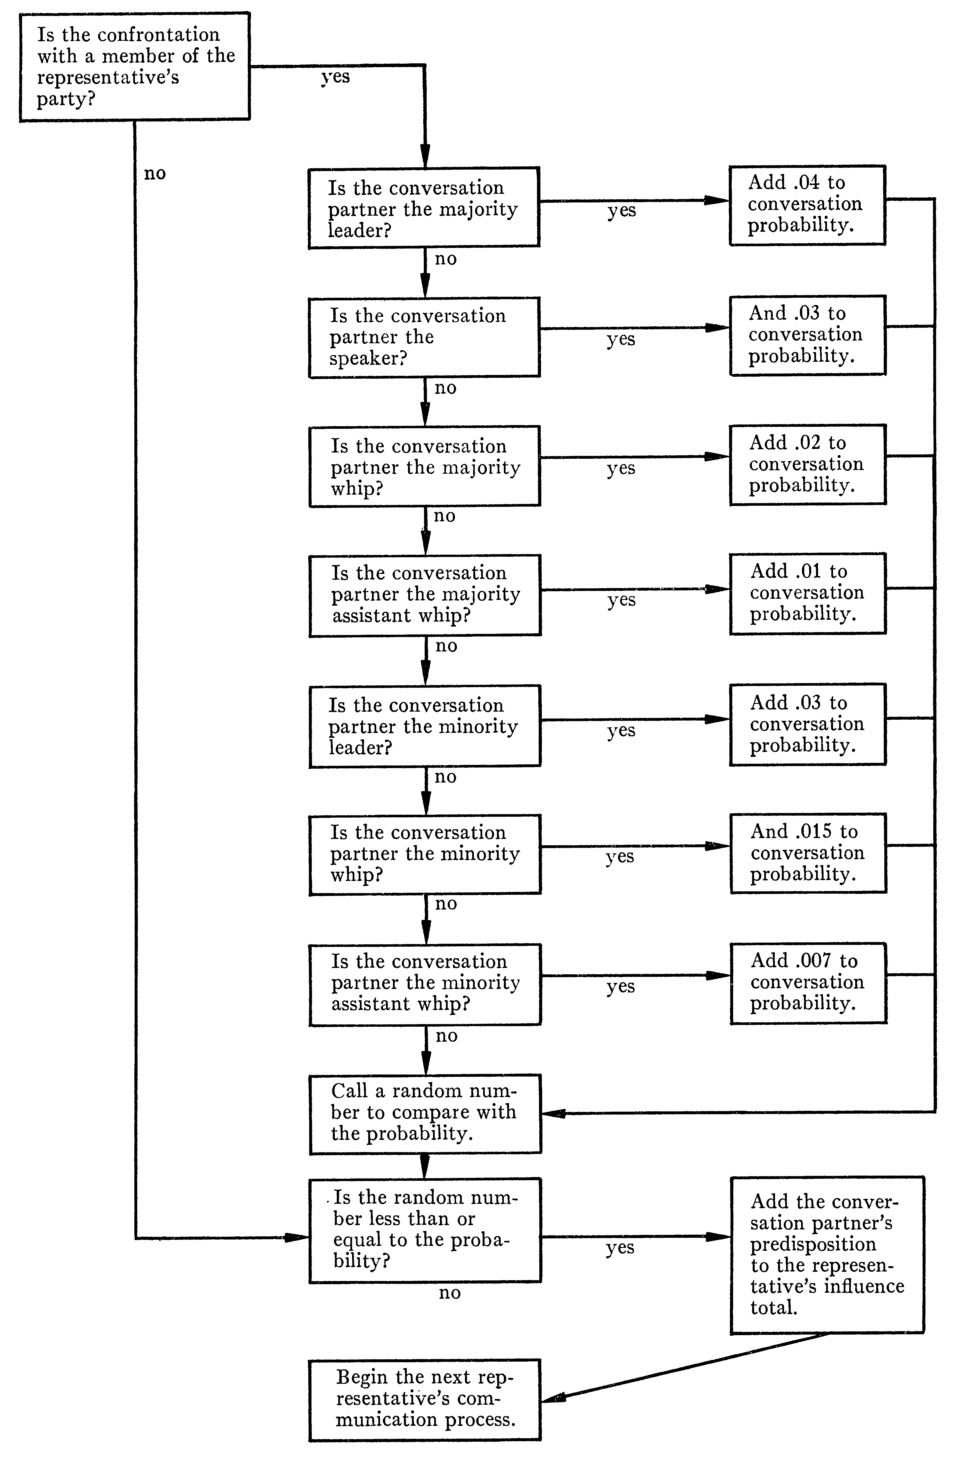
\includegraphics[height=10cm]{images/domain_spesific_model.png} 
\caption{Toimialakohtaisen mallin simulaation eräs osa \citep{Shapiro1968}}
\label{fig:domain_sim}
\end{figure}

Uudempi simulaatioperinne ottaa paremmin huomioon niin erilaisten toimijoiden kuin satunnaisuuden roolia. Esimerkiksi \citet{orbell2004machiavellian} arvioivat yhteistyöhön liittyvien normien kehittymistä useiden vuosisatojen aikana simuloiden normeja ja niiden vaikutusta yhteiskunnassa. Mallin perusteella Orbell et al. argumentoivat, että yhteistyön tapahtumista tukee mahdollisuus arvioida toisen toimijan tilannekuvaa ja motiiveja. Myös \citet{altaweel2012mobilizing} käyttävät agenttipohjasta simulointia poliittisten protestien simulointiin ja esittävät mallissaan arvioita erilaisten tekijöiden, kuten rahoituksen ja rangaistusten vaikutusta protestiliikkeiden muodostumisessa. Yllättävää kyllä, kummassakin tapauksessa mallin pohjalta tehtiin varsin vähän ajoja, jolloin mallien satunnaistekijät eivät välttämättä nouse luotettavasti esille. Kuitenkin, muten \citet{Villatoro2013} ovat tehneet, simulaatiota voidaan ajaa usempia kertoja -- heidän tapauksessaan 5000 kertaa -- tulosten vahvistamiseksi ja simulaation pohjalta muodostettu aineisto on myös luvattu, avoimen tieteen hengessä, tutkijoiden käyttöön. Heidänkin työnsä tarkastelee rankaisun merkitystä normien synnyssä ja ylläpitämisessä. Laajojen yhteiskunnallisten ilmiöiden simuloinnin lisäksi menetelmiä voidaan käyttää niin sairaalan organisaation ja kansanterveystyön ennustamiseen \citep{Pearson2011} kuin myös veropäätösten vaikutukseen arviointiin \citep{bloomquist2006comparison}.

Agenttipohjaisen mallinnuksen lisäksi satunnaistekijöitä voidaan huomioida Monte Carlo--simuloinnilla -- jolloin ei niinkään mallinneta yksittäisen agentin toimintaa ja vuorovaikutusta vaan käytetään yksinkertaisempaa mallia ilmiöstä. Sovelluskohteina on ollut esimerkiksi äänestyspäätökset \citep{quinn1999voter,jackman2000estimation} sekä sodan päättymisen ennustaminen \citep{slantchev2004initiators}.
 
\subsection{Agenttipohjainen malli}

\begin{figure}
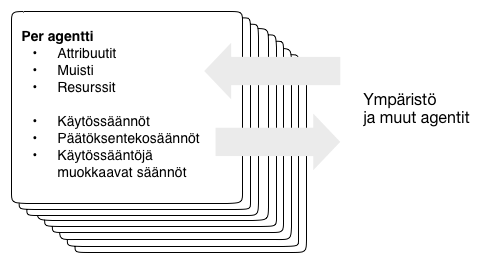
\includegraphics[height=3cm]{images/agenttimalli.png} 
\caption{Agenttipohjainen simulaatio \citet{Macal2009} mukaan}
\end{figure}

Agenttipohjaisesissa malleissa (\textit{agent-based models, ABM}) mallinnetaan yhteisön toimintaa yksittäisten toimijoiden kautta. Kukin toimija, eli agentti, on yksilöllinen toimintaheuristiikka, tai prefrenssifunktio. Tämän preferenssifunktion sekä mahdollisen satunnaisfuntion avulla määritellään agentin tila seuraavalla ajanhetkellä: \begin{equation}\mathcal{T}_{i,(t+1)} = \mathcal{P}( \mathcal{T}_{i,t} ) + \varepsilon \label{abm:yhtälö}\end{equation} Toistamalla sama simulaatio järjestelmän kaikille agenteille, voidaan määrittää järjestelmän tila ajanhetkellä $t+1$ ajanhetken $t$ perusteella. Luonnollisesti preferenssifuntio $\mathcal{P}$ voi ottaa huomioon myös muiden agenttien toimeinpiteet ja tästä syntyneen järjestelmän tilan tehdessään päätöstä tulevasta tilasta \citep[esimerkiksi][]{Bonabeau2002}. \todo{toinen lähde?} Mallinnusprosessia siis joudutaan etukäteen määrittelemään merkittäviä muuttujia, joka \citet{Gilbert1993} mukaan helpottaa teorioiden muodostamista ja testaamista: simuloidussa malleissa kun ei voida ottaa huomioon kaikki yhteiskunnallista ilmiötä kuvaavia muuttujia.

\citet{Bonabeau2002} kuvaa tarkemmin agenttipohjaisen mallien hyötyjä. Hänen mukaansa agenttipohjainen mallinnus havaitsee paremmin nousevia ilmiöitä {\textit{emergent phenomena}), eli ilmiöitä joita ei voida havaita tarkastellessa vain yksilöitä, vaan yksilöiden välinen vuorovaikutus tai toisten yksilöiden toiminta vaikuttaa yksilön käyttäytymiseen. Esimerkkeinä täläisistä tilanteista on oppiminen ja sopeutuminen (ajallinen korrelaatio), aikaisempi kokemus ja tehdyt päätökset (muisti sekä polkuriippuvuus) sekä epälineaarinen käyttäytyminen, esimerkiksi tietyn kynnysarvon jälkeen tapahtuva toiminta.

Toisena hyötynä \citet{Bonabeau2002} mainitsee agenttipohjaisen mallin helpomman tulkittavuuden. Hän arvioi, että yksilökeskeinen kuvaus toiminnasta on selkeämpi kuin erilaiset tilasiirtymäkuvaukset tai prosessikuvaukset. Tämän takia hän arvioi agenttiohjaisen mallien olevan helpommin asiantuntijoiden tulkittavissa ja arvioitavissa, jolloin mallit ovat selkeämmin validoitavissa. Lisäksi \citet{Bonabeau2002} kritisoi keskisuureiden käyttämistä ilmöiden kuvaamiseksi, koska näissä tilanteissa ääriarvot eivät ole nähtävissä ja keskisuureet tasoittavat vaihtelua.

\subsection*{Mikrosimulaatiot}

Agenttipohjaisten mallien lisäksi on mahdollista käyttää mikrosimulaatiota  (\textit{microsimulation model}). Sen toiminta ei merkittävästi eroa esitetystä yhtälöstä \ref{abm:yhtälö}, eli malli pyrkii ennustamaan yksilön toimintaa. Kuitenkin taustalla oleva lähestymistapa eroaa. Agenttipohjaisen malli pyrkii luomaan ilmiön parametrien avulla ja tämän jälkeen tarkastelemaan luomiseen tarvittuja parametreja, kun taas mikrosimulaatiossa ilmiöön liittyvät taustamuuttujat ja niiden väliset määritellään etukäteen \citep[58--59]{Gilbert2005}. Yksilökeskeisen mallinnustavan takia pidän mikrosimulaatioita ja agenttipohjaisia malleja samankaltaisina agenttipohjaisina simulaatioina, vaikka niiden toiminnan yksityiskohdat eroavatkin toisistaan.

\subsection*{Kirjastot ja kehitysympäristöt}

Agenttipohjaisen simulaation toteutukseen on olemassa useita erilaisia valmiita kirjastoja sekä alustoja. \cite{Tobias2004} esittää arviointikriteereitä onnistuneille simulaatioympäristöille: ideaalisti kehitysympäristö pystyy automaattisesti luomaan agentteja tiettyjen todennäköisyysmallien perusteella, yksittäiset agentit voivat olla monimutkaisia ja pystyvät viestimään toisilleen. Lisäksi kehitysympäristön arvioinnissa tulisi heidän mukaansa ottaa huomioon kehittäjien tarpeita, esimerkiksi asennuksen yksinkertaisuus, graafisen käyttöliittymän käyttö ja kattava dokumentaatio ovat hyvän kehitysympäristön tunnusmerkkejä. Lisäksi \citet{Tobias2004} ehdottavat avoimen lähdekoodin lisenssejä positiivisena tekijänä, koska niiden käyttö mahdollistaa mallin muutokset.

Näiden kriteerien pohjalta \citet{Tobias2004} päätyvät suosittelemaan RePast-ympäristöä. RePast sallii useamman kielen käytön simulaation kehityksessä, mikä on mahdollistanut erilaisten välineiden ja kirjastojen käytön kehityksessä \cite{North2006}, kuten esimerkiksi Javan käytön. Esimerkki Java-pohjaisesta RePast-mallista on liitteessä \ref{appedix:repast}, RePast-ympäristön hyödyn havaitsee valmiista koodista, jotka liittyvät simulaation pohjaan, siinä tehtävään etsintään ja liikkumiseen sekä todennäköisyysjakaumien käsittelyyn. Lisäksi merkitsemällä (\textit{annotate}), voidaan erikseen merkitä kuinka usein kyseinen agentti suorittaa oman preferenssifunktionsa.

\subsection{Monte Carlo--simulointi}

\section{Tekstin analysointi}
\label{sec:textanalysis}

Numeerisen aineiston lisäksi yhteiskuntatieteissä työskennellään usein tekstiaineiston kanssa, kuten haastatteluiden, viranomaistekstien sekä nykyisin myös sosiaalisen median tuotoksien kanssa. Perinteisesti aineiston analyysi on suoritettu lukemalla tekstejä ja tekemällä tästä päätelmiä, kuitenkin tämä on varsin raskasta ja onkin toivottavissa, että tietokoneistetusti tekstin luokittelua voitaisiin systematisoida -- \citet{Grimmer2013} korostavatkin, että laskennalliset menetelmät toimivat tässä kohtaa ihmisen apuna, mutta tarkoitus ei ole korvata ihmistä analysoinnissa. Tekstin analysointiin käytettäviä menetelmiä on useita, niin ohjatun kuin ohjaamattoman, koneoppimisen tekniikoita \citep[esimerkiksi][]{Grimmer2013}, kirjallisuuskatsauksen perusteella tekstiainestoa on analysoitu sentimenttianalyysillä ja aiheiden tunnistuksella.

\citet{groshek2013public} arvioivat Yhdysvaltojen vuoden 2012 presidentin vaalien aikaista viestintää sosiaalisessa mediassa. Aineistona heillä oli yli 1.4 miljoonaa viestiä, osa Facebookissa ja osa Twitterissä -- mikä kertoo tarpeesta soveltaa laskennallista menetelmää analyysissä. Analyysi suoritettiin laskemalla sanojen lukumääriä ja termejä, joihin sanat olivat yhteydessä. Erityisesti kirjoittajat tarkastelivat, kuinka ehdokkaan vastustajasta puhuttiin ehdokkaan Facebook- ja Twitter-sivuilla ja havaitsivat, ettei vastustajasta puhuttu merkittävästi negatiivisemmin kuin ehdokkaasta. Laskennallisesti kyseessä ei ole erityisen mielenkiintoinen ongelma: kuten kuvasta \ref{fig:wordnet} nähdään, analyysi perustuu sanojen ilmenemiseen toistensa kanssa ja tämän pohjalta laskettuihin todennäköisyyksiin.

\begin{figure}
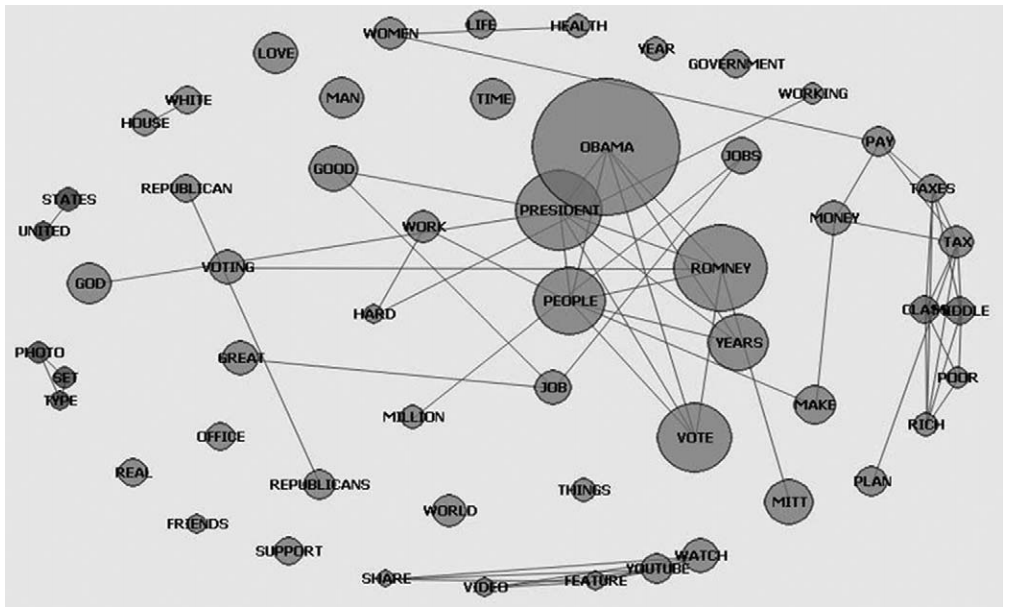
\includegraphics[height=8cm]{images/word_net.png} 
\caption{Barack Obaman sosiaalisen median sivuiden perusteella luotu kuva sanoista \citep{groshek2013public}}
\label{fig:wordnet}
\end{figure}

Laskennallisesti mielenkiintoisempaa on tekstin sisällön merkitysten arviointi, yksinkertaisimmillaan tekstin positiivisuuden ja negatiivisuuden arviointi. Jatkaen poliitikoiden sosiaalisen median tutkimusta, \citet{park2011networked} arvioivat poliitikkojen verkkoprofiilissa esiintyviä positiivisia je negatiivisia sanoja, ja havaitsevat että oppositiopuolueiden sivuilla oli enemmän positiivisia viestejä hallituspuolueisiin verrattuna. Myöskin \citet{tumasjan2010election} ovat kiinnostuneet poliitikkoihin liittyvistä viesteistä Twitterissä, he sentimenttianalyysin perusteella päättelevät, että puolueen kannattajat puhuvat kilpailevista poliitikoista negatiivisemmin kuin omasta ehdokkaastaan, mutta positiivisissa viesteissä ei nähdä selvää eroa.

Lisäksi laskennallisesti on mahdollista erottaa aiheita ja teemoja -- mikä vastaa ihmistyötä vastaavassa laadullisen tutkimuksen prosessissa. \citet{levy2013driving} ovat analysoineet lainsäädäntöön liittyneitä kommentteja ja laskennallisesti eroittaneet aineistosta teemoja, joita kommenteissa käsiteltiin. He analysoivat tarkemmin, ketkä ovat lähettäneet kommentteja ja havaitsevat eroja lobbausorganisaatioiden ja yksittäisten kansalaisten teemojen välillä. Tällä perusteella he arvioivat lainsäädäntötyön läpinäkyvyyttä ja lobbaustahojen merkittävyyttä lainsäädäntötyössä.

\subsection*{Ohjattu ja ohjaamaton oppiminen}

Sekä sentimenttianalyysi että teemojen luokittelu (\textit{topic modeling}) ovat koneoppimiseen perustuvia algoritmeja, mutta niiden toimintaperiaateet ovat erilaisia. Sentimenttianalyysi perustuu ohjattuun oppimiseen \textit{(supervised learning)}, jossa kutakin syötettä vastaa tulos (${ (s_1, t_1), \ldots , (s_n, t_n) }$). Esimerkiksi sentimenttianalyysissä tekstille on määritelty sitä vastaava sentimenttilukuarvo. Opetusvaiheessa ohjattu oppiminen laskee eri syötteiden välisiä yhteyksiä ja tällä tavalla päättelee, mitkä tekijät vaikuttavat kuhunkin tulokseen, täsmällisemmin optimoi funktiota $g$ syötteiden joukolta $\mathcal{S}$ tulosjoukolle $\mathcal{Y}$, siten että virhe on mahdollisimman pieni. Opetuksen jälkeen ohjattu oppiminen pystyy itsenäisesti arvioimaan mielivaltaista syötettä vastaavan tulosarvon käyttäen funktiota $g$.

Ohjaamattomassa oppimisessa \textit{(unsupervised learning)} ei ole opetusjaksoa, eikä aineistosta siis etukäteen tarvitse luokitella osittain. Sen sijaan näissäkin tapauksissa pyritään löytämään aineistoista virhefunktion kannalta paras tulos, mutta eri ohjaamattoman oppimisen menetelmissä virhefunktioden tyypit eroavat toisistaan.

\subsection{Sentimenttianalyysi}

Esitellyissä artikkeleissa käytössä oli yksinkertainen, sanoihin ja niiden lukumäärään perustuva sentimenttianalyysi, jossa sanoja luokitellaan jollain asteikolla ja tätä kautta muodostetaan sanakirja, jota voidaan käyttää analysoimisessa \citep{pennebaker2001linguistic,Thelwall2010}\footnote{Sentimenttianalyysiä voidaan myös tehdä myös ohjaamattomasti, tavoite on aina löytää tekstiaineistosta piirteitä joiden perusteella voidaan ennustaa kielen käyttäytymistä. Käytettyjen menetelmien joukko on laaja, esimerkiksi Bayesilaisia luokittimia ja tukivektorikoneita on vertailtu \citep{Pang02a,Pang05a,Thelwall2010}. Koska sentimenttianalyysiä tutkitaan aktiivisesti, tässä työssä esittelen yksinkertaisen toteutuksen sentimenttianalyysistä.}. Analyysiä voidaan täydentää käyttämällä laajemmin kielellisiä ominaisuuksia, kuten huutomerkejä sekä perättäisille sanoja, sekä niiden vaikutusta yksittäisten termien määrään. On myös mahdollista koneellisesti testata erilaisia yhdistelmiä ominaisuuksia, ja verrata näin saatuja arvoja ihmisen suorittamaan luokitukseen lauseiden osalta, pyrkien optimoimaan eri ominaisuuksien painoarvoja siten, että virhe ihmisen tekemän luokituksen välillä on mahdollisimman pieni \citep{Thelwall2010}.

Sentimenttianalyysi perustuu siis tekstin piirteisiin \textit{(features)} tarkasteluun, laskennallisesti mielenkiintoisempi -- tosin, \citet{Thelwall2010}\footnote{\citet{Thelwall2010} on keskittynyt sosiaalisen median viestien analysointiin MySpace--palvelussa, ja samaa menetelmää on sovellettu myös löydetyssä kirjallisuudessa.} aineiston kohdalla vähemmän tarkka -- menetelmä on tukivektorikoneiden \textit{(support vector machine)} käyttö luokittamiseen. Tukiverkkokoneet perustuvat piirrevektoreiden ja (opetettujen) arvojen pareihin ($\{ (x_1, y_1), (x_2, y_2), \ldots, (x_n, y_n) \}$, missä $x_i \in \mathbb{R}^n$ on tukivektori ja $y_i$ opetettu arvo), jotka muodostavat pinnan. Tukivektorikoneen ideana on jakaa tämä pinta mahdollisimman selvästi eri ryhmiin piirrevektoreihin liittyvällä funktiolla $f(x_i) = \beta x_i + \beta$, jolloin kyseessä on jälleen virheen vähentämiseen perustuva iteratiivinen laskentaprosessi \citep{Hastie2009}.

\subsection*{Työkalut}

Agenttipohjaisten simulaatioiden kohdalla korostettiin dokumentaatiota, avoimuutta ja muokattavuutta eri ympäristöjen arvioinnissa \citep{Tobias2004}. Sentimenttianalyysissä samanlaiset kriteerit ovat mielekkäitä: kuitenkin, koneoppimista soveltavissa lähestymistavoissa mielekästä on myös arvioida koneopitun aineiston laatua ja luotettavuutta. Esimerkiksi \citet{Thelwall2010} kehittämä SentiStrength tarjoaa valmiina käytettäväksi englannin kielelle soveltuvan sanakirjan, mutta mahdollistaa myös omien painotusten kehittämisen ja optimoinnin.

\subsection{Teemojen luokittelu}

Toisin kuin yllä esitetty sentimenttianalyysi, teemojen luokittelu on ohjaamatonta koneoppimista, jonka voi yksinkertaisimmillaan rakentaa latenttien Dirchlet-allokaatioihin \textit{(latent Dirchlet allocation, LDA)} perustuen. Ideana on siis, että aineistolla on piilossa olevia tekijöitä, joita voidaan havainnoida välillisesti aineistosta \citep{Blei2010}. 

\subsection*{Työkalut}

\section{Säänönmukaisuuksien ja ryhmien löytäminen}
\label{unsupervised}

Perinteinen politiikan tutkimuksen teema on selittää eroja valtioiden välillä, esimerkiksi demokratian tilan arviointia taustamuuttujien perusteella. \citet{Jurek2013} jatkavat tätä perinteistä linjaa selittämällä valtioiden demokaattisuutta Freedom House --aineiston ja taustamuuttujien, kuten uskonnon ja demokratian keston perusteella. Menetelmänä he käyttävät työssään assosiaatiosääntöjen hakua laskennallisesti, jonka perusteella he löysivät yhteensä 210 erilaista sääntöä. Lisäksi he nostavat esille, että koneoppimisen soveltaminen mahdollistaa selittävien tekijöiden muutoksien valitsemisen vapaammin kuin perinteisten tilastollisten mentelmien soveltaminen, jossa tarkasteltavien sääntöjen määrä on yleisesti merkittävästi pienempi.

%% \citet{Leskovec2010} regressio-classifier

\cite{collingwood12}

%% Marketing Segmentation Through Machine Learning Models An Approach Based on Customer Relationship Management and Customer Profitability Accounting

%% Kaufman and Rousseeuw (1990)

Ohjaamatonta koneoppimista voi lähestyä useilla erilaisilla menetelmillä, kuten assosiaatiosäännöillä, dimensioiden vähentämisellä (\textit{dimensionality reduction}) sekä  klusteroimalla \citet[485--586]{Hastie2009}\footnote{\citet[43--138]{Hastie2009} nostavat myös regressiomallit koneoppimisen osana, mutta kuten johdannossa argumentoin kyseessä on yhteiskuntatieteen näkökulmasta enemmänkin perinteinen laskennallinen menetelmä, enkä siksi esittele tarkemmin näiden yksinkertaisten mallien käyttöä osana laskennallista yhteiskuntatiedettä.}. \todo{Lisää johdattelua?}

\subsection{Assosiaatiosäännöt}

Assosisaatiosäännöt perustuvat aineiston ominaisuuksien käsittelyyn siten, että ne selittävät mahdollisimman suuren osan aineistossa havaituista eroista. Kustakin säännöstä lasketaan erikseen sen selitysaste, mutta myös luottamus kyseisen säännön yleistettävyyteen ja säännön nosto (\textit{lift}), jolla arvioidaan löydetyn säännön merkittävyyttä \citep[485--586]{Hastie2009}. Eräs algoritmi sääntöjen muodostamiseksi on \citet{Agrawal1994a} esittelemä Apriori. Apriori laskee eri sääntökombinaatioiden frekvenssin aineistosta, ja tällä perusteella määrittelee mitkä säännöt ovat tarpeeksi yleisiä yleistämiseksi. \todo{pseudoalgoritmin esittely? pitäisi linkata jotenkin laskennan tulos luottamukseen ja lifteihin}

\begin{algorithm}
\State $S_1$ = {kaikki yhden alkion kokoiset säännöt}
\State $i = 2$

\While{ $S_{i-1} \neq \emptyset$ }
  \State $E_i = \mathtext{ehdokkaat}(S_{i-1}) $

	\ForAll{siirtyma \in $E_i$}
		\State $e.maara += |\{e' \in E_i | e' = siirtyma \}|$
	\EndForAll  
  
  \State $S_i = \{e \in E_i | e.maara \geq tuki \}$
\EndWhile

\Return $\cup_i S_i$
\end{algorithm}


\subsection{Klusterointi}

Dimensioiden vähentämisellä viitataan prosessiin, jossa ilmiötä kuvaavien muuttujien määrää vähennetään etsimällä muuttujaryhmiä, joiden kautta aineiston vaihtelua selitetään mahdollisimman hyvin. Yhteiskuntatietelijöiden yleisesti tuntema menetelmä tähän on pääkomponenttianalyysi (\textit{principal component analysysi, PCA}), jonka kautta aineisto jaetaan selittäviin faktoreihin. \todo{Lisää PCAsta?} Laskennalliset menetelmät mahdollistavat myös aineiston samankaltaisten alkioiden esittämisen ryhminä, eli klusteroinnin. Menetelmiä klusterointiin on useita, esimerkiksi $k-means$ sekä spektriklusterointi\todo{Spectral Clustering} \citep[485--586]{Hastie2009}.

k-means-menetelmä pyrkii, nimensä mukaisesti, löytämään keskiarvon kullekkin klusterille ja valitsemaan klustereiden sijainnit siten, että havaintojen sijoittaminen näille keskiarvopisteille aiheuttaa mahdollisimman pienen virheen. Kyseessä on iteratiivinen algoritmi, jota toistetaan kunnes klustereiden sijainnit eivät vaihdu. \todo{pseudokoodia?} Vastaavasti spektriklusterointi perustuu samankaltaisten ominaisarvojen ryhmittämistä, jolloin klusterit korostavat samankaltaisten ominaisuuksien joukkoja paremmin kuin keskiarvoon perustuva k-means klusterointi.


\section{Keskustelu}

\subsection{Validiteetti haasteena}

Niin määrällisessä kuin laadullisessa yhteiskuntatieteessä tutkimuksen laatua arvioidaan validiteetin ja reliabiliteetin kannalta. Ensimmäinen viittaa ulkoiseen laatuun, eli siihen tutkitaanko ilmiötä oikein ja jälkimmäinen sisäiseen laatuun, eli onko tutkimus tehty uskottavasti.

Sentimenttianalyysi, teemojen luokittelu, assosiaatiosääntöjen oppiminen sekä klusterointi ovat aineiston käsittelyyn tarkoitettuja algoritmeja, jolloin uskottavuuden kannalta keskeisempää on aineiston laatu: onko aineiston mahdollinen esikäsittely suoritettu oikein ja onko aineisto kerätty oikein. Iteratiivissa algoritmeissa -- kuten klusteroinnissa -- on tarpeen myös tarkastella tulosten pysyvyyttä eri aloitusarvoilla, eli arvioida saadun tuloksen herkkyyttä \todo{two-solution-problem paperi EDMStä?}.

Kirjallisuuden pohjalta laskennallisen yhteiskuntatieteen käytetyn menetelmä oli simulointi, joka on mielestäni uskottavuuden kannalta myös haastavin. Toisin kuin yllä mainituissa menetelmissä, simuloinnissa menetelmä ja käytettyjen parametrien määrä voi vaikuttaa tulokseen. \citet{bloomquist2006comparison} on työssään arvioinut kolmea julkaistua agenttipohjaista mallia, havaiten ettei tuloksia näissä malleissa ole verrattu ilmiöstä kerättyyn aitoon aineistoon. Lisäksi  hän kritisoi sitä, ettei malleilla ole suoritettu useampia ajoja, jolloin mallien tuloksiin liittyy tiettyä epävarmuutta. Samoin \citet{edmonds2005computational} arvioivat erilaisia simulointimalleja, nostaen esille huolensa toistettavuudesta sekä ymmärryksen mallin rajoituksista ja soveltuvuudesta eri teemoihin.

Kritiikki on mielestäni osuvaa ja osoittaakin suurimman huoleni simulaatiotutkimukseen: kuinka voidaan varmistaa, että esitetyt simulaatiot aidosti vastaavat varsin monimutkaisia yhteisöjen käyttäytymissääntöjä? Viimeaikaisessa simulaatiotutkimuksessa näihin kritiikkeihin on pyritty vastaamaan, esimerkiksi simulaatiomalli voidaan rakentaa ilmiötä tutkivien koeasetelmien valossa \citep{Villatoro2013} tai mallien tuloksia voidaan verrata olemassa oleviin ilmiöihin aktiivisesti ja käyttää näitä mallin rakennuksen tukena \citep{Pearson2011}.

Simulaatiomallit heikkouksistaan huolimatta tarjoavat kiinnostavia mahdollisuuksia mallin luomiseen vuorovaikutuksessa laskennallisten sekä yhteiskuntatieteilijöiden ja muiden toimijoiden välillä. \citet{Milne2014} kuvaavat prosessia, jossa simulaatiomallia ja sen tuloksia arvioitiin yhdessä virkamiesten ja tutkijoiden välillä. Heidän mukaansa mahdollisuus muuttaa mallia lisäsi yhteisymmärrystä ilmiöstä ja helpotti tiedon siirtämistä tutkijoilta soveltajille. Toisaalta, kuten \citet{Saunders-Newton2001a} huomauttavat, eri henkilöt suhtautuvat laskennallisiin menetelmiin myös erilaisin odotuksin. Tällöin luottamuksen rakentaminen ja laskennallisen menetelmän läpinäkyvyys ja selkeys ovat merkittäviä arvoja osana laskennallista yhteiskuntatiedettä, kuten perinteisessä yhteiskuntatieteellisessä tutkimuksessa.

\subsection{Työskentely monitieteellisesti}

\begin{figure}

%\begin{subfigure}{.6\textwidth}
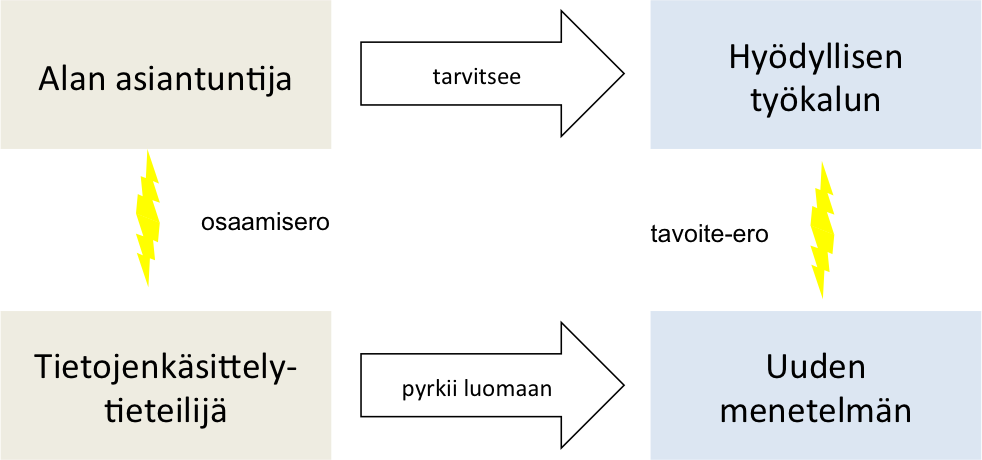
\includegraphics[width=.6\textwidth]{images/monitieteellisyys_ongelma.png} 
\caption{Menetelmäkehityksen ero soveltajaan \citep[mukaillen][7]{Wijk2006}}
\label{fig:domain_expert_vs_computation_specialist}
%\end{subfigure}
%~~
%\begin{subfigure}{.2\textwidth}
%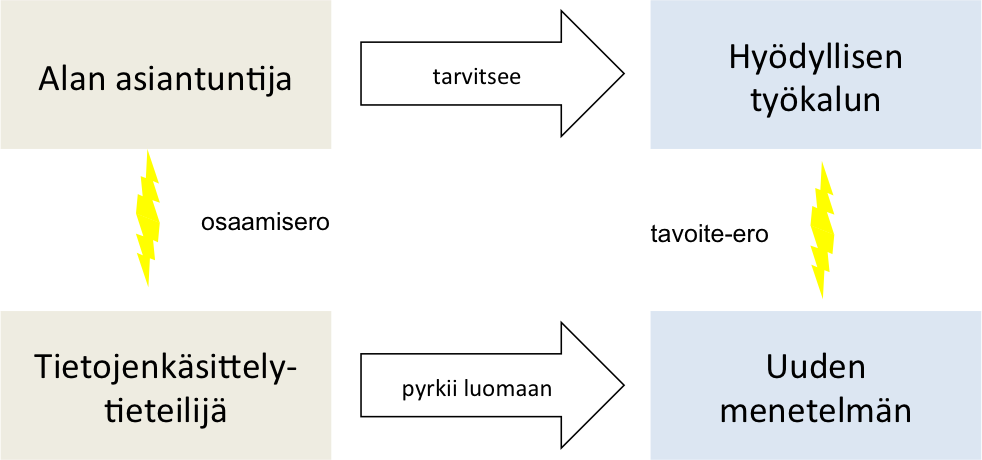
\includegraphics[width=\textwidth]{images/monitieteellisyys_ongelma.png} 
%\caption{Menetelmäkehityksen ero soveltajaan \citep[mukaillen][7]{Wijk2006}}
%\end{subfigure}

\end{figure}

Tutkimuksen uskottavuuden kohdalla nostin esille jo haasteen yhteistyöstä laskennallisen ja yhteiskuntatieteen välillä. \citet{Wijk2006} käsittelee monitieteellistä yhteistyötä visualisoinnissa. Oman kokemuksensa pohjalta hän huomauttaa, että alan asiantuntijalla (\textit{domain expert}) ja visualisaation tutkijalla on usein erilaiset tavoitteet visualisaation kehittämisessä: kun visulisaation tutkija ensisijaisesti kehittää uusia visualisaatiomenetelmiä, niin alan asiantuntijan tavoitteena on hyödyllisen työkalun kehittäminen -- mikä voidaan saavuttaa myös perinteisillä menetelmillä. Kuvassa \ref{fig:domain_expert_vs_computation_specialist} esitän saman erottelun sovellettuna laskennalliseen yhteiskuntatieteeseen, alan asiantuntijan ja tietojenkäsittelytietelijöiden välisenä tarkasteluna.

\citet{Wijk2006} jatkaa, että tavoite-eron takia yhteistyön muoto on joku seuraavista: tietojenkäsittelytieteen asiantuntija voi hänen mukaansa toimia työvälinekehittäjänä tai jatkaa tietojenkäsittelyn menetelmien kehittämistä. Tietojenkäsittelytieteen asiantuntija voi myös soveltaa käyttäjäkeskeisiä menetelmiä kehitystyössään, jolloin laskennallisia menetelmiä kehitetään yhteistyössä alan asiantuntijan kanssa. Toisaalta, tietojenkäsittelyttieteen asiantuntija voi myös itse tutustua alaan tai kehittää visualisaatiotekniikoita aiheisiin, joista hän on kiinnostunut. van Wijk kutsuu viimeistä yhteistyön muotoa mielenkiintovetoiseksi kehitystavaksi (\textit{curiosity driven}), ja nostaa esille muodon haasteen: sellaisenaan tällä toimintatavalla ei voida ratkaista aihealueen haastavimpia ongelmia. Näin laskennallisen yhteiskuntatieteen mahdollisiksi... \todo{johtopäätös: yhteiskuntatieteessä voidaan tehdä UCD tai toolsmith}

\subsection{Paradigman muutos?}

Kuten \citet[265]{watts11} esittääkin

\begin{quote}
\texttt{[o]}n kuitenkin välttämätöntä soveltaa kaikkia näitä \texttt{[sekä laskennallisia että kuvailevia]} lähetymistapoja samanaikaisesti, pyrkien saavuttamaan johtopäätöksiä siitä, kuinka ihmiset käyttäytyvät ja kuinka maailma toimii -- sekä ylhäältä että alhaalta, käyttäen hyödyksi kaikkia menetelmiä jotka ovat käytettävissä. (\textit{oma suomennus})
\end{quote}

Laskennallisille menetelmille yhteiskuntatieteissä on siis tarvetta, koska niiden avulla on mahdollista esittää ratkaisuja uusiin kysymyksiin. Kuitenkin, samaan aikaan tulee huomioida yhteiskuntatieteiden oppihistoria monimenetelmäisenä ja -paradigmaisena: eri lähestymistapojen käyttö samojen ongelmien käsittelyyn on perinteinen menetelmä yhteiskuntatieteiden osalta. Tämän takia monitieteelliinen työskentely on tarpeen, mutta valitettavasti tällä hetkellä laskennallinen yhteiskuntatiede ei yleisesti keskustele 

\section{Johtopäätökset (2)}

Työssä käsiteltiin laskennallisia menetelmiä yhteiskuntatieteiden toiminnassa, ja tätä kautta muodostunutta laskennallisen yhteiskuntatieteen toimikenttää. Työn ensimmäinen kontribuutio käsittelee toimintakentän määritelmää: tässä työssä käytettiin varsin rajaavaa määritelmää laskennallisesta yhteiskuntatieteestä (katso sivu \pageref{css-maar}), missä korostettiin laajojen tietomassojen käyttöä ennustavien mallien luomiseksi. Kuitenkin, laskennallinen yhteiskuntatiede voidaan nähdä laajemmin, esimerkiksi \citet{cioffi-revilla10} esittää huomattavasti tätä laajemman määritelmän, ja halutessa esimerkiksi moderni tilastotiede täyttää monia laskennallisuudelle asetettuja oletuksia: elaboroi. Tämän takia dikotomisen asettelun sijaan on mielekästä puhua laskennallisen yhteiskuntatieteen jatkumosta. elaboroi.

Toinen merkittävä kontribuutio pohtii laskennallisen yhteiskuntatieteen asemaa alana. Korostin tarvetta poikkitieteelliseen työskentelyyn, missä sekä laskennallisten menetelmien asiantuntijat että kohdealueen asiantuntijat työskentelisivät yhdessä. Lisää. Arvioin myös, muodostaako laskennallinen lähestymistapa paradigman muutoksen yhteiskuntatieteissä... Kuitenkin, ilmeistä on, että laskennallisuus on uusi väline, joka on käytettävissä yhteiskuntatieteessä. lisää...

Lisäksi työssä on esitelty kolmea laskennallista menetelmää tarkemmin ...

% \section*{Kiitokset}

% Kiitän työn ohjaajaa, Antti Ukkosta, keskusteluista ja kyseenalaistavista kysymyksistä. Lisäksi kiitän Airi Lampista sekä Eric Malmia työn aikana käydyistä keskusteluista sekä \texttt{pamee}ta irkkiavautumisien kuuntelusta.


\newpage

\bibliographystyle{abbrvnat}
\addcontentsline{toc}{section}{Lähteet}
\bibliography{bsc,/Users/mnelimar/Dropbox/_tools/library.bib} 

\newpage

\appendix

\section{RePast-esimerkki}
\label{appedix:repast}

\lstinputlisting[language=Java,breaklines=true,numbers=left,tabsize=1]{examples/RePast.java} 

RePast-dokumentaation pohjalta luotu esimerkki.

%% http://repast.sourceforge.net/docs/RepastJavaGettingStarted.pdf

\end{document}
